%                                                                 aa.cls
% A&A submission draft — Gaia DR3 asteroid close-encounter catalogue.
% Compile: pdflatex -> bibtex -> pdflatex x2  (needs aa.cls + aa.bst from
% https://www.aanda.org/for-authors/latex-issues/texnical-informations).
% See README.md in this directory.
\documentclass{aa}

\usepackage[utf8]{inputenc}
\usepackage{graphicx}
% amstext (not full amsmath) provides \text without redefining \iint, so it
% coexists with txfonts, the Times-look font package A&A recommends.
\usepackage{amstext}
\usepackage{txfonts}
\usepackage{hyperref}

% Figures live one level up (docs/figures/); for actual submission copy them
% into this directory and drop the graphicspath line.
\graphicspath{{../figures/}}

\begin{document}

\title{An all-pairs catalogue of real three-dimensional close encounters
between numbered main-belt asteroids during the Gaia DR3 window, with a
measured incompleteness budget}

\titlerunning{A catalogue of real 3D asteroid close encounters (Gaia DR3)}
\authorrunning{D. Frascarelli}

% -------------------------------------------------------------------------
% TODO(author): fill in author list, affiliations, ORCID and contact e-mail
% before submission. Placeholders below.
% -------------------------------------------------------------------------
\author{D.~Frascarelli\inst{1}}

\institute{%
  Affiliation --- TODO
  \email{dsanfra@gmail.com}
}

\date{Received --- ; accepted ---}

% A&A structured abstract: context / aims / methods / results / conclusions.
\abstract
% context
{Close approaches between asteroids are the classical route to asteroid mass
determination and a dynamical observable of the main belt. Systematic encounter
searches exist --- from early surveys \citep{galad2002} to mutual-encounter
catalogues built for Gaia astrometry \citep{ivantsov2018} and the
signal-ranked search behind the largest mass catalogue to date
\citep{fuentesmunoz2025} --- but their event lists are published truncated
(top candidates per perturber) or without a characterised selection function:
no all-pairs 3D encounter catalogue has been published in full with provenance
and a \emph{measured} incompleteness budget.}
% aims
{We build a systematic catalogue of real 3D close encounters between numbered
main-belt asteroids (semi-major axis 1.5--4.0\,AU) during the Gaia DR3 window
(2014 July 25 -- 2017 May 28), publish it in full, and, unlike a
bulk propagation exercise, we \emph{measure} what the detection pipeline misses
rather than asserting completeness.}
% methods
{Orbits are propagated from a single frozen MPCORB snapshot centred on the
window. Encounters are found by a per-timestep 3D KD-tree spatial query and
refined on a dense temporal sub-grid. Reported distances use an analytic
two-body refiner; a hybrid variant carries full N-body (rebound/ASSIST)
refinement for the dynamically fragile (low-perihelion or high-eccentricity)
subset. Perturber masses come from a joint mass$+$orbit least-squares fit to
Gaia FPR astrometry.}
% results
{The catalogue records the minimum physical 3D separation --- a genuine spatial
approach, not a sky-plane co-location --- for 72\,236\,904 candidate pairs within
0.05\,AU, with encounter epoch, relative velocity, geometry, and estimated
physical properties. Its distinguishing feature is a \emph{measured}
completeness budget: the Kepler-to-N-body refinement error (median
12\,$\mu$AU, p99 2.5\,mAU) and the threshold-induced false-negative rate
(0.70\,\%, symmetric and scatter-dominated) bound this catalogue directly, while
the recall of an orbital prefilter on the adverse tail (76\,\%) is quantified as a
caveat for prefiltered runs. Applied to mass determination, the
engine recovers all four calibrator masses (Ceres, Vesta, Pallas, Hygiea) at
$|z|<3$ and determines sixteen perturbers, of which ten identifiable masses
agree with recent independent work.}
% conclusions
{The catalogue is a reusable, defensibly characterised target-selection
resource for asteroid dynamics and mass determination. It is explicitly not
complete, and no new large--large encounter or unpublished large-body mass
emerged from the numbered population.}

\keywords{minor planets, asteroids: general --
          celestial mechanics --
          astrometry --
          catalogs --
          surveys --
          methods: data analysis}

\maketitle

% =========================================================================
\section{Introduction}
\label{sec:intro}

Close encounters between asteroids are of interest on several fronts. A slow,
close approach between a massive perturber and a small test body deflects the
latter's orbit measurably, and such events are the classical route to asteroid
mass determination \citep{michalak2000, fienga2003, goffin2014, baer2017,
siltala2020, li2023, fuentesmunoz2025}. Encounters between members of the same
dynamical family probe the collisional history of the belt, and the statistical
distribution of mutual approach distances and velocities is itself a dynamical
observable.

Systematic encounter searches have a long history. \citet{galad2002} searched
for mass-determination encounters across 24\,599 asteroids;
\citet{ivantsov2018} built a catalogue of mutual encounters of the numbered
population over 2013--2023 specifically to exploit Gaia astrometry;
\citet{goffin2014} fitted masses against the entire numbered population rather
than curated target lists; and \citet{fuentesmunoz2025} ran a systematic,
signal-ranked search over 1\,783 perturbers against more than a million
orbits --- using, for main-belt targets, the same 0.05\,AU threshold adopted
here. What none of these works provides is the \emph{event list published in
full with a characterised selection function}: published tables are truncated
to the top candidates per perturber, and the completeness of the underlying
searches is asserted rather than measured. That is the gap this work fills: an
\emph{all-pairs} catalogue over the numbered main-belt population
($1.5 \le a \le 4.0$\,AU) in the Gaia DR3 window, published in full with
provenance, where --- the point that separates this catalogue from a bulk
propagation exercise --- we \emph{measure} what the detection pipeline misses
rather than asserting completeness.

A methodological distinction is central. Two asteroids can appear arbitrarily
close in right ascension and declination as seen from Earth while remaining
astronomical units apart along the line of sight. This catalogue detects the
former case only when it is also the latter: it records the \emph{minimum
physical separation in three dimensions} between the two bodies' heliocentric
positions, independent of any observer. It is therefore a catalogue of genuine
spatial approaches, not of sky-plane co-localisations. Light-time correction
--- essential when comparing model positions to Gaia's astrometry --- is
deliberately \emph{not} applied here, because the encounter is a purely
geometric relation between two propagated trajectories at a common dynamical
time.

The remainder of this paper describes the data and detection method
(Sect.~\ref{sec:method}), the measured completeness budget that is the
catalogue's distinguishing feature (Sect.~\ref{sec:completeness}), the notable
individual events surfaced by mining the catalogue (Sect.~\ref{sec:notable}),
the application to mass determination (Sect.~\ref{sec:mass}), data availability
(Sect.~\ref{sec:data}), and conclusions (Sect.~\ref{sec:conclusions}).

% =========================================================================
\section{Data and method}
\label{sec:method}

\subsection{Sources and conventions}
\label{sec:sources}

Orbital elements are taken from a single frozen MPCORB snapshot,
\texttt{MPCORB\_20160217.DAT} (SHA-256 prefix \texttt{3e44e7d3\ldots}), selected
because its osculating epoch lies at the centre of the Gaia DR3 window,
minimising the propagation distance --- and hence the accumulated two-body
error --- for Kepler refinement. The snapshot hash and download date are
recorded in the catalogue's provenance sidecar so that results are traceable to
an exact input; MPCORB is a living file and results are not bit-reproducible
across snapshot versions. The run is restricted to \emph{numbered asteroids}
(higher orbital quality); provisional designations are out of scope for this
release.

The temporal domain brackets the Gaia DR3 Solar System survey period
\citep{tanga2023}: the propagation window is 2014 July 25 -- 2017 May 28, whose
start (the DR3 astrometric-solution baseline) slightly precedes the 2014 August 5
start of nominal SSO operations, so the window fully contains the survey coverage.
All internal computation is
carried out in Julian Date on the Barycentric Dynamical Time (TDB) scale;
conversions to/from the Barycentric Coordinate Time (TCB) that Gaia reports,
and to UTC, are performed only at input/output interfaces. Distances are in AU,
angles in radians, and velocities in AU/day internally, converted to
user-facing units (km, degrees, km\,s$^{-1}$) only for output.

\subsection{Detection}
\label{sec:detection}

The naive cost is prohibitive: $\sim$150\,000 bodies over a multi-year window at
hour-level cadence implies of order $10^{10}$ pairwise distances per step.
Detection is therefore layered.

An \emph{orbital prefilter} is available to prune pairs that cannot physically
approach --- the shipped heuristic keeps a pair only if $|\Delta a|\leq0.5$\,AU
and $|\Delta i|\leq30\degr$. This filter is a deterministic mask on osculating
elements. We note here, and quantify in Sect.~\ref{sec:prefilter}, that at
main-belt scale ($\gg5000$ bodies) the pair-list prefilter is not built; the
frozen run therefore applied only the KD-tree spatial query, and the
$|\Delta a|$ cut did \emph{not} shape this catalogue (provenance
\texttt{prefilter.effective = "skipped\_large\_n"}).

The core of the detector is a \emph{per-timestep 3D KD-tree}. At each coarse
step the heliocentric ecliptic positions of all bodies are inserted into a
KD-tree ($O(N\log N)$ construction), and a radius query returns neighbour
candidates ($O(\log N)$ per query), avoiding any $O(N^2)$ distance matrix. The
coarse cadence is $\Delta t = 12$\,h. To prevent the cadence from missing an
encounter whose true minimum falls \emph{between} two samples, the query radius is
\emph{widened} to $r_q = 0.05\,\mathrm{AU} + v_{\max}\,\Delta t \approx
0.0572$\,AU with $v_{\max} = 25$\,km\,s$^{-1}$: under near-linear relative motion a
pair whose separation dips below 0.05\,AU between samples is within $r_q$ at the
nearer bracketing sample and therefore enters the candidate set; the sub-grid
refinement then discards any whose true minimum exceeds 0.05\,AU. Bracketing a
minimum midway between two samples strictly requires only $v_{\max}\,\Delta t/2
\approx 0.0536$\,AU; the pipeline uses the full-step widening ($v_{\max}\,\Delta
t$), a factor-of-two conservative margin. The bracketing is thus exact for
relative velocities up to $v_{\max}$, and the residual (encounters with
$v_{\rm rel} > v_{\max}$) is bounded in Sect.~\ref{sec:prefilter}.

Each coarse candidate is then \emph{refined on a dense temporal sub-grid}: a
$\pm2$\,h window around the apparent minimum is sampled at 120\,s, and the
minimum separation, encounter epoch, and relative velocity are extracted from
the refined track. Time blocks are independent, so the scan parallelises across
processes.

\emph{Propagation} is two-tiered. The coarse KD-tree scan is driven by an
N-body rebound integration (WHFast; Sun\,+\,Jupiter\,+\,Saturn; $dt = 1$\,h).
The sub-grid refinement that produces the \emph{reported} minimum distance runs
through an analytic two-body Kepler propagator. Over the short Gaia DR3 arc
($\sim$3\,yr from the central epoch) two-body propagation is adequate for the
bulk of the belt, and its residual error is measured, not assumed
(Sect.~\ref{sec:refineerror}). For the dynamically fragile subset --- pairs
with perihelion $q_{\min}<1.8$\,AU or eccentricity $e_{\max}>0.3$, 8\,728\,509
pairs (12.08\,\% of the catalogue) --- a \emph{hybrid} catalogue replaces the
Kepler distances with full N-body refinement (rebound IAS15; Sun\,+\,8
planets\,+\,4 major asteroids; $\pm12$\,h around the Kepler minimum; 60\,s
sampling). The hybrid catalogue carries
$\mathrm{refinement\_method}\in\{\mathrm{kepler},\mathrm{nbody}\}$ per row
together with the Kepler and N-body values and their residuals, so users needing
sub-mAU geometry on high-$e$ / NEA-crossing pairs can cite it directly.
Universal N-body refinement of all 72\,M pairs ($\sim$400 CPU-days) is
explicitly out of scope: the median error outside the fragile subset is already
below 1\,mAU (Sect.~\ref{sec:refineerror}), so the marginal gain does not
justify the cost.

\subsection{Characterisation}
\label{sec:characterisation}

For each detected pair the catalogue records the minimum separation and its
exact epoch (from the refined sub-grid), the relative velocity at closest
approach, and the geometry of the event relative to Gaia --- solar elongation
and an observability flag --- computed on the characterised catalogue. Of the
72\,236\,904 encounters, 13\,640\,870 (18.9\,\%) fall in a Gaia-observable
configuration. Physical properties (absolute magnitude $H$, and diameter and
taxonomic class estimated from $H$ with a class-dependent albedo when no direct
measurement exists) are attached to both bodies. Diameters derived this way are
order-of-magnitude estimates, not measurements, and any size-based selection
inherits that uncertainty.

The two encountering bodies are treated as independent test particles moving in
the planetary\,+\,massive-asteroid field; their \emph{mutual} gravitational
deflection over the approach is not modelled. At asteroid masses and the
$\gtrsim10^5$\,km separations that dominate the catalogue this is entirely
negligible for the recorded geometry, and it is in any case the very quantity a
downstream mass determination sets out to measure, not a property of the
encounter itself.

\subsection{Catalogue overview}
\label{sec:overview}

The parent population and the encounter statistics are summarised in
Figs.~\ref{fig:sep}--\ref{fig:aei}. The minimum-separation distribution
(Fig.~\ref{fig:sep}) rises monotonically toward the 0.05\,AU threshold, as
expected for a roughly uniform spatial density of encounter geometries; the
relative-velocity distribution (Fig.~\ref{fig:relvel}) peaks near its median of
4.25\,km\,s$^{-1}$, typical of main-belt crossing velocities. The orbital
distribution of the 93\,010 encountering bodies (Fig.~\ref{fig:aei}) reproduces
the belt's known structure --- the 3:1, 5:2 and 2:1 Kirkwood gaps appear as
clear voids --- confirming the sample is the ordinary numbered population, not a
biased subset.

\begin{figure}
  \centering
  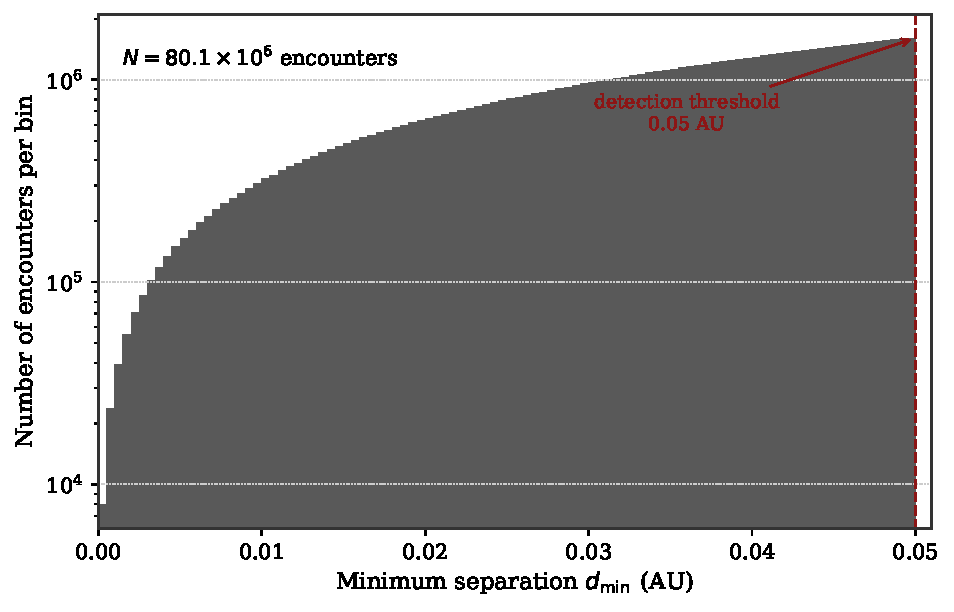
\includegraphics[width=\hsize]{fig1_separation_hist.pdf}
  \caption{Distribution of minimum 3D separations for the
  $72.2\times10^{6}$ catalogued encounters (log count per bin). The dashed line
  marks the 0.05\,AU detection threshold.}
  \label{fig:sep}
\end{figure}

\begin{figure}
  \centering
  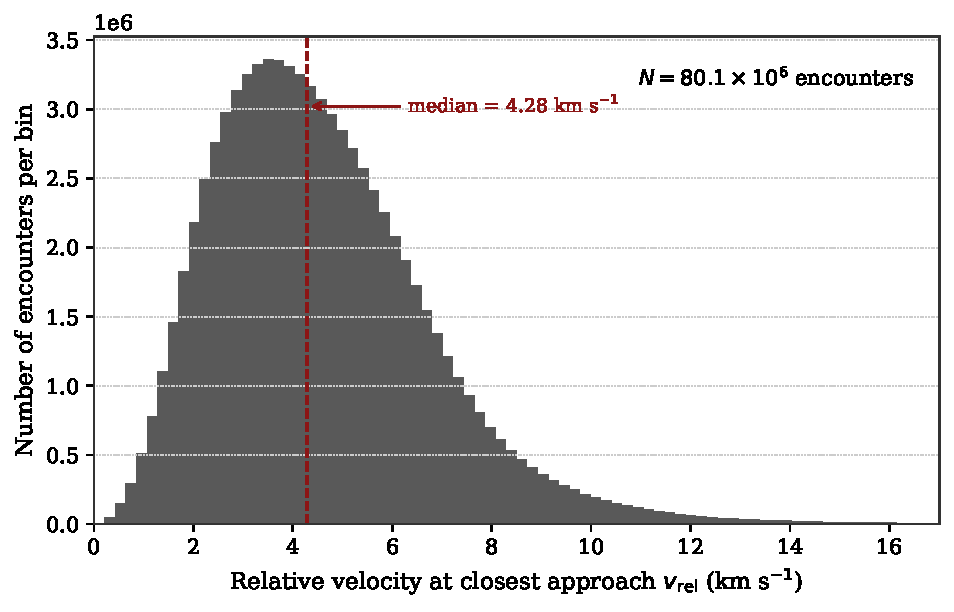
\includegraphics[width=\hsize]{fig2_relvel_hist.pdf}
  \caption{Distribution of relative velocity at closest approach; the median is
  4.25\,km\,s$^{-1}$.}
  \label{fig:relvel}
\end{figure}

\begin{figure}
  \centering
  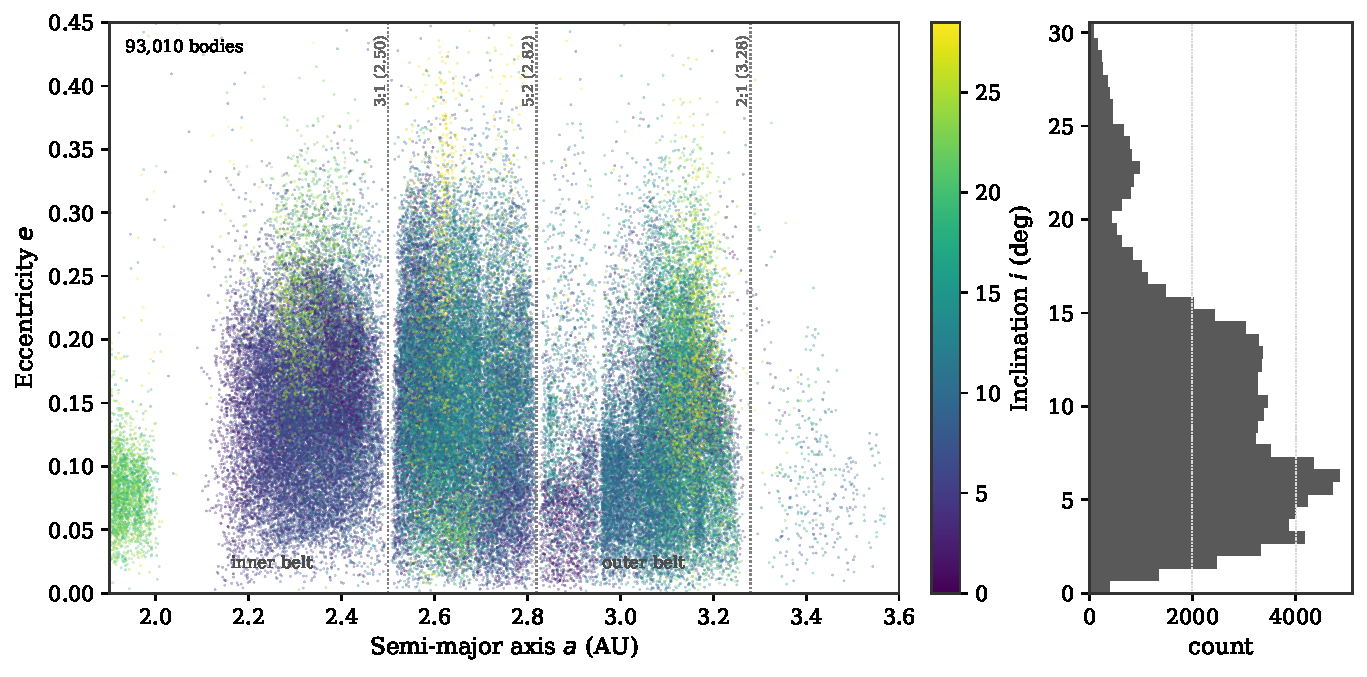
\includegraphics[width=\hsize]{fig3_aei_map.pdf}
  \caption{Semimajor axis vs eccentricity of the 93\,010 encountering bodies,
  coloured by inclination, with the inclination marginal at right. The 3:1, 5:2
  and 2:1 mean-motion resonances (Kirkwood gaps) are marked.}
  \label{fig:aei}
\end{figure}

% =========================================================================
\section{Completeness budget}
\label{sec:completeness}

The value of this catalogue is not that it detects encounters --- that is a bulk
propagation --- but that it states, with measured numbers, what it \emph{misses}
and how large the Kepler-vs-N-body distortion is. Three quantities are measured;
each is reproducible from a dedicated script.

\subsection{Kepler vs N-body refinement error}
\label{sec:refineerror}

The reported distances in the frozen catalogue come from the two-body refiner.
We measured the resulting error against full N-body refinement in two stages.
In \emph{Stage A} (964 stratified pairs re-refined under full N-body) the median
$|\Delta d| = 12\,\mu$AU, p95 $= 678\,\mu$AU, p99 $= 2.5$\,mAU, max
$= 11.3$\,mAU. In \emph{Stage B} (production N-body refinement of the entire
8.73\,M fragile subset) p99 $|\Delta d| = 1.99$\,mAU, max $= 15.2$\,mAU, with
0 failed integrations, 0 unconverged, and maximum energy drift
$5.6\times10^{-14}$.

For scale, 1\,mAU $\approx 1.5\times10^{5}$\,km, and the detection threshold is
0.05\,AU. The median distortion is thus $\sim$4 orders of magnitude below the
threshold, and even the Stage B worst case is $\sim$30\,\% of a threshold ---
confined to the fragile subset, which the hybrid catalogue refines. A separate
check of the truncated perturber set (the scan used only
Sun\,+\,Jupiter\,+\,Saturn) shows that adding the remaining planets shifts
closest-approach distances by a median 1.3\,$\mu$AU (p99 67\,$\mu$AU, max
80\,$\mu$AU), i.e.\ $\sim$100$\times$ below the Kepler two-body error --- the
perturber truncation is not the dominant error term.

\subsection{Threshold censoring (measured false-negative rate)}
\label{sec:censoring}

Because the catalogue contains only pairs whose \emph{Kepler} distance is below
0.05\,AU, a subtle bias arises at the threshold. When the fragile subset is
re-refined to N-body, 25\,283 pairs (0.29\,\%) cross the threshold
\emph{upward} (Kepler $<0.05$, N-body $\geq0.05$) and, by construction, none
cross downward --- a pair that Kepler placed \emph{above} 0.05\,AU was never
written, so its downward crossing \emph{cannot be observed}. The apparent
one-sided ``no false negatives'' is therefore censoring, not measurement.

We measured the missing side directly. Re-running Kepler detection at a widened
0.06\,AU threshold over 10\,000 numbered bodies --- drawn to span the belt in
$(a, e, i)$ and so representative of the propagated population --- and isolating
the 17\,469 pairs with Kepler distance in $[0.05, 0.06)$\,AU --- exactly the band a 0.05\,AU
catalogue discards --- then re-refining each under full N-body, 0.70\,\%
[95\,\% CI 0.59--0.83\,\%] cross \emph{downward} below 0.05\,AU (a conservative
floor of $\sim$0.42\,\% after excluding near-boundary cases). The residual
$\Delta d$ ($N-K$) has median $-3\times10^{-7}$\,AU and $\sigma\approx
3.7\times10^{-4}$\,AU --- a symmetric, scatter-dominated distribution, not a
directional bias. In other words the crossing is a threshold selection effect
(Eddington/Malmquist family): scatter of amplitude
$\sim$1$\sigma\approx4\times10^{-4}$\,AU pushes pairs just inside the threshold
to just outside, and their mirror images (just outside to just inside) fall
outside the catalogue. The upward rate ($\sim$1.5\,\% in the boundary bin
$[0.045, 0.050)$) and the downward rate ($\sim$0.4--0.7\,\% in $[0.05, 0.06)$)
are consistent with a single symmetric process. Crossings concentrate in
low-$q$ / high-$e$ / fast orbits, exactly where two-body propagation is
weakest --- which independently validates the $q_{\min}<1.8 \lor e_{\max}>0.3$
subset criterion.

Extrapolated catalog-wide (order-of-magnitude, the $[0.05, 0.06)$ band scaling
as $N^2$), this implies of order $10^5$ real $<0.05$\,AU encounters censored by
the Kepler cut ($\sim$1.5--2.5$\times10^5$), separate from and additional to the
prefilter recall deficit of Sect.~\ref{sec:prefilter}. This is why the word
``complete'' is never used for this catalogue.

\begin{figure}
  \centering
  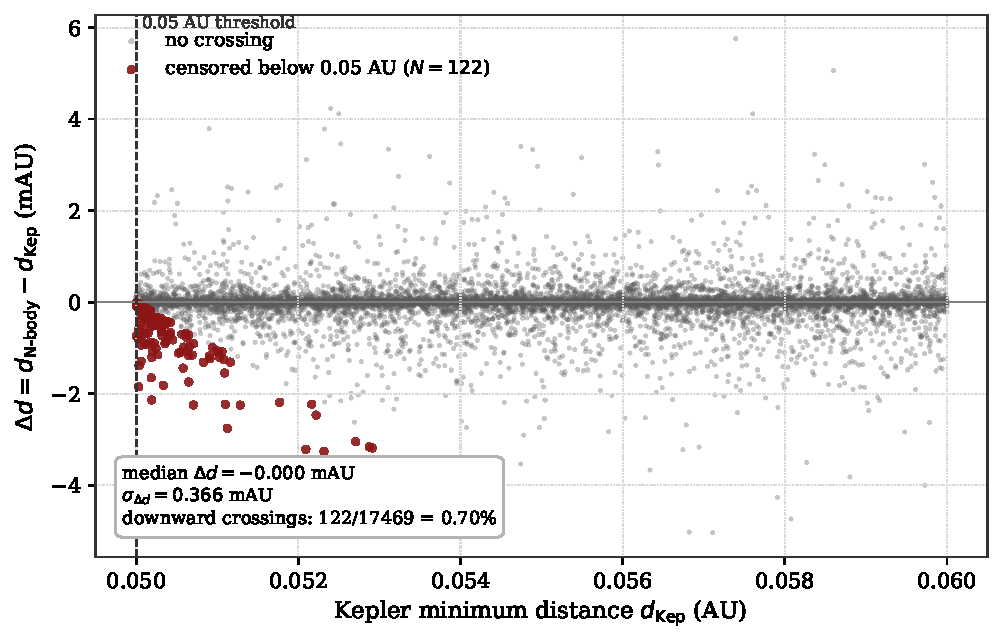
\includegraphics[width=\hsize]{fig4_kepler_nbody_threshold.pdf}
  \caption{Threshold censoring, measured directly. For the 17\,469 pairs with
  Kepler distance in $[0.05, 0.06)$\,AU --- the band a 0.05\,AU catalogue
  discards --- re-refined under full N-body, $\Delta d = d_{\rm N\text{-}body} -
  d_{\rm Kep}$ is plotted against $d_{\rm Kep}$. The distribution is symmetric
  about zero (median 0.000\,mAU, $\sigma = 0.366$\,mAU); the 122 pairs
  (0.70\,\%) that cross downward below 0.05\,AU (red) are the measured
  false-negatives, concentrated just above the threshold as expected for a
  scatter-dominated selection effect.}
  \label{fig:threshold}
\end{figure}

\subsection{Prefilter recall on the adverse tail}
\label{sec:prefilter}

The shipped $|\Delta a|\leq0.5$\,AU prefilter is blind to eccentricity: a
high-$e$ orbit reaches well inside the belt at perihelion and well outside at
aphelion, so it can physically cross an orbit whose semimajor axis differs by
far more than 0.5\,AU. We measured the damage this would cause on the adverse
subset (numbered, $a\in[1.5, 4.0]$, $e>0.3 \lor i>15\degr$; 52\,411 bodies),
exploiting the fact that the prefilter is a pure deterministic mask: running
detection without the prefilter and intersecting with the mask is
byte-identical to running with it. Ground truth is 606\,393 real
adverse--adverse encounters $<0.05$\,AU; the prefilter keeps 463\,164, for a
recall of 76.38\,\% [95\,\% CI 76.27--76.49\,\%]. Thus 143\,229 encounters would
be missing from a prefiltered catalogue (a lower bound --- adverse--normal pairs
were not measured), and 99.6\,\% of that loss is the $|\Delta a|$ cut alone.
Recall degrades smoothly with eccentricity, from $\sim$99.9\,\% below $e=0.1$ to
$\sim$39\,\% above $e=0.7$.

Two points bound the impact. First, an eccentricity-aware
\emph{radial-overlap} prefilter --- keep a pair iff its threshold-padded
heliocentric radial ranges $[a(1-e), a(1+e)]$ overlap --- is a provable
necessary condition for a $<0.05$\,AU encounter, is just as cheap, and recovers
100\,\% recall on the adverse subset; it is the recommended replacement for any
future run. Second, and specific to \emph{this} freeze: because the run was at
main-belt scale the pair-list prefilter was skipped entirely, so the
$|\Delta a|$ cut did not actually drop these pairs from the frozen catalogue.
The 76\,\% figure measures the damage the prefilter \emph{would} cause if
applied at small $N$, not damage suffered here. Completeness of this freeze is
instead bounded by the threshold censoring of Sect.~\ref{sec:censoring}. The 12\,h
coarse cadence does \emph{not} by itself lose encounters up to
$v_{\rm rel} = v_{\max} = 25$\,km\,s$^{-1}$, because the widened query radius
(Sect.~\ref{sec:detection}) brackets them; the only encounters it can miss have
$v_{\rm rel} > 25$\,km\,s$^{-1}$, and just 0.0012\,\% of catalogued encounters
exceed that (p99.99 $= 20$\,km\,s$^{-1}$, max 68\,km\,s$^{-1}$), so the residual
cadence-induced incompleteness is $\lesssim 10^{-3}$\,\% --- three orders of
magnitude below the threshold-censoring term and negligible. For the dynamically cold bulk of the belt (low $e$,
small $\Delta a$) recall is $\sim$99.9\,\%; the incompleteness is a property of
the high-$e$/high-$i$ tail, which any science touching NEA-crossing or high-$e$
pairs must cite.

\subsection{Recovery of literature encounter pairs}
\label{sec:litrecovery}

As an external check we cross-matched the signal-ranked (perturber, target)
pairs that \citet{fuentesmunoz2025} used for mass determination against this
catalogue. Of 40\,176 numbered pairs drawn from their per-perturber target
lists, 11\,842 (29.5\,\%) appear as $<0.05$\,AU encounters in the hybrid
catalogue. This fraction is a lower bound and, crucially, the non-recovery is
dominated by a \emph{domain difference}, not a detection failure: 91.6\,\% of
the unmatched pairs have both bodies present in the catalogue but never
approached within 0.05\,AU \emph{inside the 2.8-yr DR3 window}. For main-belt
targets \citet{fuentesmunoz2025} apply the same 0.05\,AU threshold used here,
but they search over the full observational arcs (decades, through late 2024),
so a pair whose close encounter falls outside 2014--2017 cannot appear in this
catalogue.
% TODO(regen, Tarea 11): cuantificar sobre el catálogo regenerado cuántos de
% los 25,962 pares no recuperados tienen su encuentro FM fuera de la ventana.
A further 8.4\,\% are targets or perturbers outside
the numbered, propagated universe (high or provisional designations), and ---
the decisive point --- 0\,\% are pairs that our catalogue contains but places
beyond 0.05\,AU. In other words, every literature pair that is genuinely a
$<0.05$\,AU encounter and lies in the numbered population is recovered; the
apparent shortfall is entirely pairs that are not $<0.05$\,AU encounters or not
numbered. Per-body recovery among the most-listed perturbers ranges from 6\,\%
(Davida) to 61\,\% (Liguria), with the Ceres and Vesta calibrators at
$\sim$36\,\%. Pair-level cross-matching against \citet{goffin2014} is not
applicable: Goffin's masses come from a single \emph{simultaneous} global fit of
all perturber masses to the astrometric residuals of the entire numbered
population, not from per-perturber target lists, so there is no set of
(perturber, target) pairs to match (the VizieR tables give per-perturber masses
and literature mass compilations only).

% =========================================================================
\section{Notable events}
\label{sec:notable}

Mining the characterised catalogue surfaces individual events across four axes.
We stress at the outset that the value of these tables is statistical and
archival rather than a single headline discovery: there is no new large--large
($D\gtrsim100$\,km) encounter --- the two such events in the catalogue are both
already known --- and every candidate below is under the frozen two-body
assumptions and requires N-body revalidation before publication. Distances are
physical 3D separations at closest approach; diameters are $H$-derived
estimates.

\subsection{Large--large encounters}
\label{sec:largelarge}

Only two encounters have both bodies with estimated $D\gtrsim100$\,km, and both
involve already-studied bodies (Table~\ref{tab:dd100}). The population of
both-$D\gtrsim50$\,km encounters is richer (Table~\ref{tab:dd50}). The closest
both-$D\gtrsim50$\,km event, (305) Gordonia $\times$ (830) Petropolitana at
$9.9\times10^5$\,km, involves neither of the sixteen studied perturbers and is a
natural target for N-body revalidation.

\begin{table*}
\caption{The two encounters with both bodies $D\gtrsim100$\,km.}
\label{tab:dd100}
\centering
\begin{tabular}{llccccc}
\hline\hline
body 1 & body 2 & date (UTC) & dist (km) & $v_{\rm rel}$ & $D_1$ & $D_2$ \\
       &        &            &           & (km/s)        & (km)  & (km)  \\
\hline
(1) Ceres & (57) Mnemosyne & 2017-01-10 & $6.5\times10^6$ & 7.25 & 763 & 139 \\
(7) Iris  & (44) Nysa      & 2014-08-13 & $7.3\times10^6$ & 5.35 & 281 & 139 \\
\hline
\end{tabular}
\end{table*}

\begin{table*}
\caption{Encounters with both bodies $D\gtrsim50$\,km, top ten by minimum
distance.}
\label{tab:dd50}
\centering
\small
\begin{tabular}{llccccc}
\hline\hline
body 1 & body 2 & date (UTC) & dist (km) & $v_{\rm rel}$ & $D_1$ & $D_2$ \\
       &        &            &           & (km/s)        & (km)  & (km)  \\
\hline
(305) Gordonia   & (830) Petropolitana & 2014-09-18 & $9.88\times10^5$ & 3.28 & 62.6 & 53.8 \\
(426) Hippo      & (788) Hohensteina   & 2015-04-17 & $1.15\times10^6$ & 8.82 & 73.5 & 64.6 \\
(145) Adeona     & (780) Armenia       & 2016-11-09 & $1.50\times10^6$ & 6.34 & 84.0 & 56.3 \\
(739) Mandeville & (415) Palatia       & 2017-04-05 & $1.70\times10^6$ & 8.36 & 70.9 & 51.1 \\
(675) Ludmilla   & (80) Sappho         & 2016-02-15 & $1.71\times10^6$ & 2.97 & 93.0 & 90.0 \\
(51) Nemausa     & (91) Aegina         & 2016-07-13 & $2.08\times10^6$ & 4.42 & 120  & 60.6 \\
(46) Hestia      & (482) Petrina       & 2016-07-12 & $2.46\times10^6$ & 4.23 & 75.6 & 60.6 \\
(758) Mancunia   & (740) Cantabia      & 2016-08-13 & $2.63\times10^6$ & 3.70 & 82.9 & 53.8 \\
(739) Mandeville & (754) Malabar       & 2016-03-14 & $2.72\times10^6$ & 5.26 & 70.9 & 51.6 \\
(200) Dynamene   & (1304) Arosa        & 2014-12-25 & $2.85\times10^6$ & 7.88 & 79.2 & 51.3 \\
\hline
\end{tabular}
\end{table*}

\subsection{Extreme events}
\label{sec:extreme}

The absolute closest approaches in the catalogue are between small bodies, at
separations of $\sim$1000--7000\,km (Table~\ref{tab:closest}). At these
separations two-body propagation is most fragile, so these are precisely the
events most in need of N-body revalidation; those that survive are the
geometrically most striking events in the dataset.

The slowest encounters (relative velocity down to $\sim$6\,m/s, with at least
one body $D\gtrsim5$\,km; Table~\ref{tab:slowest}) are the natural targets for
future mass determination, since a low $v_{\rm rel}$ prolongs the gravitational
interaction and enlarges the deflection. The combined ``large\,+\,slow\,+\,close''
set (one body $D\gtrsim50$\,km, $v_{\rm rel}\leq1$\,km/s, dist $\leq10^6$\,km;
Table~\ref{tab:largeslowclose}) is of the highest physical interest, being the
configuration that maximises measurable deflection.

\begin{table*}
\caption{The five closest approaches in the catalogue.}
\label{tab:closest}
\centering
\small
\begin{tabular}{llccccc}
\hline\hline
body 1 & body 2 & date (UTC) & dist (km) & $v_{\rm rel}$ & $D_1$ & $D_2$ \\
       &        &            &           & (km/s)        & (km)  & (km)  \\
\hline
(153222) 2000 YD43 & (238587) 2004 YX3  & 2016-03-11 & 1094 & 6.90 & 2.82 & 1.78 \\
(15072) Landolt    & (387599) 2001 XF180 & 2014-12-08 & 1760 & 5.87 & 3.24 & 1.62 \\
(270730) 2002 QE130 & (366918) 2005 UC211 & 2016-05-29 & 2291 & 3.10 & 1.62 & 1.18 \\
(117065) 2004 KD9  & (439086) 2011 QP5  & 2015-07-27 & 2535 & 8.25 & 3.72 & 1.86 \\
(52249) 1981 EK21  & (408138) 2013 CL75 & 2016-11-17 & 2590 & 3.16 & 3.39 & 1.41 \\
\hline
\end{tabular}
\end{table*}

\begin{table*}
\caption{The five slowest encounters (at least one body $D\gtrsim5$\,km).}
\label{tab:slowest}
\centering
\small
\begin{tabular}{llccccc}
\hline\hline
body 1 & body 2 & date (UTC) & dist (km) & $v_{\rm rel}$ & $D_1$ & $D_2$ \\
       &        &            &           & (km/s)        & (km)  & (km)  \\
\hline
(3791) Marci    & (110964) 2001 UW170  & 2017-01-18 & $5.85\times10^6$ & 0.006 & 13.5 & 2.46 \\
(47042) 1998 WP3 & (99861) Tscharnuter & 2014-07-27 & $6.03\times10^6$ & 0.015 & 5.63 & 3.24 \\
(7203) Sigeki   & (73664) 1981 EE34    & 2015-02-28 & $7.07\times10^6$ & 0.031 & 8.14 & 1.48 \\
(3384) Daliya   & (309262) 2007 RZ93   & 2016-12-20 & $4.44\times10^6$ & 0.031 & 6.17 & 1.23 \\
(7479) 1994 EC1 & (14954) 1996 DL      & 2017-05-12 & $7.10\times10^6$ & 0.032 & 6.46 & 3.09 \\
\hline
\end{tabular}
\end{table*}

\begin{table*}
\caption{The ``large\,+\,slow\,+\,close'' set (one body $D\gtrsim50$\,km,
$v_{\rm rel}\leq1$\,km/s, dist $\leq10^6$\,km).}
\label{tab:largeslowclose}
\centering
\small
\begin{tabular}{llccccc}
\hline\hline
body 1 & body 2 & date (UTC) & dist (km) & $v_{\rm rel}$ & $D_1$ & $D_2$ \\
       &        &            &           & (km/s)        & (km)  & (km)  \\
\hline
(135) Hertha      & (281202) 2007 FE47  & 2016-09-18 & $4.56\times10^5$ & 0.579 & 80.3 & 1.02 \\
(371) Bohemia     & (14711) 2000 CG36   & 2016-05-14 & $5.92\times10^5$ & 0.982 & 64.0 & 5.90 \\
(83) Beatrix      & (170676) 2003 YE180 & 2014-09-18 & $6.10\times10^5$ & 0.684 & 65.8 & 2.14 \\
(678) Fredegundis & (200373) 2000 QH89  & 2015-03-13 & $6.27\times10^5$ & 0.964 & 55.8 & 2.04 \\
(9) Metis         & (345254) 2005 UT477 & 2016-10-30 & $7.14\times10^5$ & 0.979 & 197  & 1.23 \\
(639) Latona      & (10793) Quito       & 2014-12-18 & $7.27\times10^5$ & 0.604 & 81.4 & 10.7 \\
(16) Psyche       & (139485) 2001 PT14  & 2015-01-19 & $9.66\times10^5$ & 0.869 & 235  & 2.57 \\
(7) Iris          & (153539) 2001 SD101 & 2015-08-17 & $9.97\times10^5$ & 0.806 & 281  & 2.35 \\
\hline
\end{tabular}
\end{table*}

\subsection{Same-region pairs (family proxy)}
\label{sec:family}

Pairs whose osculating elements are mutually close ($\Delta a/a\leq1$\,\%,
$\Delta e\leq0.02$, $\Delta i\leq1\degr$) \emph{and} that had a physical close
approach are candidate co-orbital / same-family associations. This is a
proximity proxy in \emph{osculating} elements, not a classification in proper
elements, and flags rather than confirms family membership. The closest such
pair, (200764) 2001 XP3 $\times$ (131597) 2001 XT2, passed within 49\,511\,km on
2014-08-13 with nearly identical $(a, e, i)$ --- $a\approx2.29$\,AU,
$e\approx0.19$, $i\approx25\degr$ for both --- a plausible genetic pair worth
follow-up in proper-element space.

\subsection{Candidate perturbers beyond the studied sixteen}
\label{sec:candperturbers}

Ranking large bodies ($D\gtrsim100$\,km) \emph{not} among the sixteen studied
perturbers by their number of \emph{useful} encounters ($v_{\rm rel}\leq3$\,km/s
and dist $\leq3\times10^6$\,km) yields the best prospects for a mass
determination the frozen mass runs have not yet attempted
(Table~\ref{tab:candperturbers}). (9) Metis heads the list with 37 useful events
and a best pair at $v_{\rm rel} = 0.38$\,km/s; (29) Amphitrite is the largest
($D\approx240$\,km) with a close $3.2\times10^5$\,km approach. These candidates
directly informed the F4 mass determination of Sect.~\ref{sec:mass}.

\begin{table*}
\caption{Large bodies outside the studied sixteen, ranked by useful encounters.}
\label{tab:candperturbers}
\centering
\small
\begin{tabular}{lccccc}
\hline\hline
body & $D$ (km) & class & useful & best dist (km) & min $v_{\rm rel}$ (km/s) \\
\hline
(9) Metis       & 197 & MBA & 37 & $7.14\times10^5$ & 0.378 \\
(30) Urania     & 109 & --  & 36 & $4.40\times10^5$ & 0.817 \\
(40) Harmonia   & 141 & --  & 36 & $6.58\times10^5$ & 1.028 \\
(19) Fortuna    & 133 & MBA & 32 & $7.43\times10^5$ & 0.678 \\
(21) Lutetia    & 120 & --  & 30 & $8.18\times10^5$ & 0.609 \\
(64) Angelina   & 104 & MBA & 30 & $8.73\times10^5$ & 0.992 \\
(44) Nysa       & 140 & --  & 30 & $8.95\times10^5$ & 0.961 \\
(20) Massalia   & 178 & --  & 28 & $8.78\times10^5$ & 0.514 \\
(29) Amphitrite & 240 & --  & 27 & $3.17\times10^5$ & 0.643 \\
(27) Euterpe    & 141 & --  & 26 & $4.63\times10^5$ & 0.847 \\
\hline
\end{tabular}
\end{table*}

\subsection{Separating new from known}
\label{sec:newknown}

A reference list of encounters touching one of the sixteen studied perturbers
(1, 2, 3, 4, 7, 10, 15, 16, 31, 52, 65, 87, 88, 107, 511, 704) is provided in
the companion material so that already-worked events can be separated from
potential discoveries. The honest verdict is that no new large--large encounter
of publication interest emerged: the belt's largest bodies are well studied, and
\citet{fuentesmunoz2025} already published over 230 masses (232 at SNR $>3$)
covering essentially all
classical large MBAs. The contribution of this work is the dataset itself --- an
all-pairs catalogue published in full with a measured completeness budget ---
demonstrated end-to-end by the mass-determination application of
Sect.~\ref{sec:mass}, not a single spectacular event.

% =========================================================================
\section{Application to mass determination}
\label{sec:mass}

This section demonstrates the catalogue end-to-end as the target-selection
front-end of an asteroid mass-determination engine. It is a \emph{usage
demonstration}, not a claim of new or improved masses: as noted below and in
Sect.~\ref{sec:newknown}, every mass recovered here is already published, and a
single out-of-sixteen perturber with $\sim$50 Gaia-FPR targets yields only a
coarse determination. Perturber mass is obtained by a joint least-squares
fit of the perturber's mass and the orbits of its test bodies --- those with a
$<0.05$\,AU encounter drawn directly from the catalogue --- over the full arc of
Gaia FPR astrometry \citep{gaiafpr2023}. The force model is ASSIST
\citep{holman2023} on the JPL DE440 ephemeris \citep{park2021}, with EIH
relativistic corrections and sixteen massive asteroid perturbers; the
fitting layer (observation model, partials, least squares) is implemented in
this work on top of rebound/ASSIST \citep{rein2012, rein2015ias15, holman2023}
and astropy \citep{astropy2022}.

\paragraph{Calibrators.} The four calibrator masses are recovered at $|z|<3$
against the literature (Table~\ref{tab:calibrators}). With $N\geq20$ test bodies,
the fit/literature ratios of Ceres \citep{park2016}, Vesta
\citep[DAWN;][]{russell2012} and Hygiea \citep{vernazza2020} fall in
$[0.943, 0.990]$ (mean bias $-4$\,\%);
Pallas, limited to 6 encounters in the catalogue, gives ratio 1.240
($z=+2.67$).

\begin{table}
\caption{Calibrator masses recovered by the joint orbit+mass fit. The $z$ column
uses the total (formal $\oplus$ systematic) $\sigma$.}
\label{tab:calibrators}
\centering
\begin{tabular}{lccccc}
\hline\hline
body & $N$ & fitted mass (kg) & $\sigma_{\rm tot}$ & ratio fit/lit & $z$ \\
\hline
Ceres  & 28 & $8.96\times10^{20}$ & 4.6\,\% & 0.955 & $-1.01$ \\
Vesta  & 28 & $2.44\times10^{20}$ & 4.6\,\% & 0.943 & $-1.30$ \\
Hygiea & 20 & $8.22\times10^{19}$ & 5.7\,\% & 0.990 & $-0.13$ \\
Pallas & 6  & $2.54\times10^{20}$ & 7.0\,\% & 1.240 & $+2.67$ \\
\hline
\end{tabular}
\end{table}

\paragraph{FOV-block covariance.} Each Gaia focal-plane crossing yields $\sim$7
CCD observations ($\sim$5\,s apart) with correlated residuals. Treating them as
independent underestimates $\sigma(\mathrm{mass})$ by a factor 1.66 (effective
$N\approx0.36\,N$). The measured intra-crossing correlation is ICC $= 0.32$; we
whiten each crossing with a block covariance
$C = \mathrm{diag}(\sigma_{\rm AL}^2) + s_c^2\,\mathbf{1}\mathbf{1}^{\mathsf T}$,
the correlated floor $s_c$ calibrated by bisection to $\chi^2_{\rm red} = 1$.

\paragraph{Sixteen perturbers.} The engine determines all sixteen. Only (16)
Psyche reaches calibrator-grade precision outside the calibrators:
$M = 2.43\times10^{19}$\,kg, $\sigma_{\rm stat} = 3.3$\,\%, $N = 36$,
$\chi^2_{\rm red} = 0.99$, ratio 1.020 vs DE441 and 1.014 ($z=+0.25$) vs the
independent \citet{fuentesmunoz2025} FPR fit. Six perturbers whose deflection
sits below the per-encounter astrometric noise return ratios in $[0.39, 0.72]$:
this is the mass$\leftrightarrow$orbit degeneracy (the fit reproduces the
astrometry with a smaller mass and a re-adjusted orbit --- regression toward zero
mass), and for these the formal Fisher $\sigma$ underestimates the error.

\paragraph{External $\sigma$ by jackknife.} Because the formal $\sigma$ scales as
$1/\sqrt{N}$ and ignores the mass$\leftrightarrow$orbit regression seen only by
leaving encounters out, we report a jackknife $\sigma$ that reincorporates it.
It is systematically 2--3$\times$ the formal $\sigma$. Its diagnostic value is
visible in the calibrators themselves: Pallas and Vesta --- whose true masses are
known --- sit at $|z|>3$ under the formal $\sigma$ but within $|z|<3$ under the
jackknife $\sigma$, showing the formal bar is genuinely too tight rather than the
jackknife being permissive. Cross-checking the ten \emph{measured}
(identifiable, $\mathrm{snr_{jack}}\geq3$) perturbers against
\citet{fuentesmunoz2025}, 10/10 fall within $|z|<3$ under the jackknife
$\sigma$, versus 5/10 under the formal $\sigma$ (6/6 vs 3/6 for the
non-calibrators, the genuinely independent comparison). The remaining perturbers
are flagged \texttt{not\_identifiable} --- their deflection does not clear the
per-encounter noise and their masses are reported as explicit bounds, not
measurements.

\paragraph{Beyond the sixteen.} The engine is not restricted to the sixteen
ephemeris perturbers: each perturber is integrated as a massive rebound particle
from its own orbital elements, so a seventeenth body outside \texttt{sb441-n16}
is added as a seventeenth massive particle with no double-counting (the ASSIST
\texttt{ASTEROIDS} force is deliberately excluded). This was demonstrated on
(19) Fortuna --- orbit fixed from JPL Horizons, mass free --- which fits with
$\chi^2_{\rm red} = 0.977$ and $M = 1.13\times10^{19}\pm2.2\times10^{18}$\,kg.
The methodological gate is green: the engine generalises to bodies beyond the
ephemeris set. Fortuna is not itself a new mass (it appears in
\citealt{goffin2014} and \citealt{fuentesmunoz2025}), and its 20\,\% $\sigma$
makes it a coarse determination consistent with the literature within the
jackknife bar ($z=+1.25$). The catalogue's top ranked out-of-sixteen candidate,
(9) Metis (37 useful encounters, Sect.~\ref{sec:candperturbers}), was run as a
second out-of-sixteen case and fits with $\chi^2_{\rm red} = 0.981$ and
$M = 4.74\times10^{18}\pm1.53\times10^{18}$\,kg (55 targets, jackknife
$\sigma = 32$\,\%), a ratio of 0.73 against \citet{fuentesmunoz2025}
($6.48\times10^{18}$\,kg), consistent within the jackknife bar ($z=-1.14$).
Fortuna and Metis thus scatter to either side of the literature ($+30$\,\% and
$-27$\,\% in central value) but both remain consistent once the honest external
$\sigma$ is used --- confirming the method generalises while underscoring that a
single out-of-sixteen perturber with $\sim$50 Gaia-FPR targets yields only a
coarse (20--30\,\%) determination, not a competitive mass. Neither is a new
mass: both are already in \citet{fuentesmunoz2025}.

We tested whether the mean $-4$\,\% calibrator bias is an artefact of an
incomplete perturber background by enlarging it from the sixteen ephemeris
bodies to thirty-five --- adding the twenty most massive asteroids of
\citet{fuentesmunoz2025} ($\approx1.6\times10^{20}$\,kg spread across the belt),
with masses from their Table 5 and orbits from JPL Horizons, using the same
custom-perturber machinery. The calibrator masses shift by $<0.25$\,\% (Ceres
$-0.02$\,\%, Vesta $-0.23$\,\%, Hygiea $+0.18$\,\%), three orders of magnitude
below the deficit being probed; the systematic floor $f_{\rm sys}$ does not drop
(4.16\,\% $\to$ 4.26\,\%). Background incompleteness is therefore \emph{not} the
origin of the $-4$\,\% bias --- a far-field, dispersed perturber population
averages to nearly zero deflection over the target ensemble. The residual bias is
more plausibly attributable to per-target orbit imperfection over the short Gaia
arc or unmodelled per-encounter astrometric systematics.

\paragraph{Relation to other methods.} The estimator used here (a joint
orbit$+$mass least-squares fit with an FOV-block covariance, an external
jackknife $\sigma$, and an identifiability flag) is functionally a transparent
reimplementation of established encounter-based mass determination, not a new
methodology. \citet{siltala2020} obtain full Bayesian posteriors by MCMC, which
natively expose multi-modality and non-Gaussian tails that a single covariance
cannot; \citet{fuentesmunoz2025} propagate a prior to a posterior over the same
Gaia FPR astrometry. Relative to those, our contribution in this section is not
methodological sophistication but end-to-end demonstration that the open
all-pairs catalogue feeds a mass pipeline whose every step (target selection,
covariance model, jackknife, identifiability cut) is open and reproducible.
Because \citet{fuentesmunoz2025} fits the same FPR data, the cross-check below is
a consistency test between two analyses of one dataset, not an independent
confirmation.

% =========================================================================
\section{Data availability}
\label{sec:data}

The primary product is the Kepler-refined candidate catalogue,
\texttt{encounters\_catalog\_rebound\_005au.parquet} (72\,236\,904 rows, SHA-256
\texttt{b0272be7\ldots}), a typed Parquet file with a machine-readable
provenance sidecar recording the MPCORB snapshot hash, the frozen configuration,
and the pipeline parameters. The derived \emph{hybrid} catalogue,
\texttt{encounters\_catalog\_hybrid\_stageb.parquet}, carries per-row
$\mathrm{refinement\_method}\in\{\mathrm{kepler},\mathrm{nbody}\}$ and both the
Kepler and N-body distances, epochs, velocities, and their residuals; it should
be cited for any science depending on sub-mAU geometry. The characterised
catalogue, \texttt{encounters\_characterized\_full.parquet}, adds observability,
solar elongation, magnitudes, diameters, and taxonomic classes for the full
72\,M rows. Anything derived from the catalogue must cite both the freeze
(catalog SHA \texttt{b0272be7\ldots}) and the code commit at its own generation
time.
% TODO(author): register the catalogue in a public archive (Zenodo/VizieR) and
% insert the DOI here before submission.

% =========================================================================
\section{Conclusions}
\label{sec:conclusions}

We have built and characterised a systematic catalogue of 72\,236\,904 real 3D
close encounters ($<0.05$\,AU) between numbered asteroids during the Gaia DR3
observation window. Unlike prior encounter-based work, which selects individual
events by hand, the catalogue is exhaustive over the numbered population and ---
its distinguishing feature --- comes with a \emph{measured} completeness budget
rather than an assumed one: the two-body refinement error (median 12\,$\mu$AU,
p99 2.5\,mAU), the threshold-induced false-negative rate (0.70\,\%, symmetric
and scatter-dominated, implying $\sim$$10^5$ censored encounters catalog-wide),
and the orbital prefilter recall on the adverse high-$e$/high-$i$ tail (76\,\%,
with a zero-cost radial-overlap fix that recovers 100\,\%). A hybrid variant
provides N-body-grade geometry on the dynamically fragile subset.

The catalogue is a working target-selection front-end for mass determination: a
joint orbit+mass fit on Gaia FPR astrometry recovers the calibrators, determines
the studied perturbers, and generalises to bodies beyond the ephemeris set,
demonstrated end-to-end (Sect.~\ref{sec:mass}). We are explicit about the
limits: distances are candidates under frozen two-body assumptions except on the
N-body-refined subset, the catalogue is not complete, and no new large--large
encounter or unpublished large-body mass emerged --- the belt's massive bodies
are already well surveyed, and the mass layer is a demonstration of use rather
than a source of competitive new masses. The contribution is the dataset itself:
an all-pairs catalogue published in full with a quantified incompleteness budget,
fed to a mass pipeline whose every step (FOV-block covariance, external jackknife
$\sigma$, identifiability flag) is open and reproducible --- a transparent
reimplementation of established encounter-based mass determination
\citep{siltala2020, fuentesmunoz2025}, not a new methodology.

\begin{acknowledgements}
% TODO(author): acknowledgements, funding, software (astropy, rebound, ASSIST,
% polars, scipy), and Gaia/DPAC boilerplate.
This work has made use of data from the European Space Agency (ESA) mission
\emph{Gaia} (\url{https://www.cosmos.esa.int/gaia}), processed by the \emph{Gaia}
Data Processing and Analysis Consortium (DPAC).
\end{acknowledgements}

\bibliographystyle{aa}
\bibliography{references}

\appendix

% =========================================================================
\section{Catalogue column schema}
\label{sec:schema}

Table~\ref{tab:schema} documents the columns of the characterised catalogue
(\texttt{encounters\_characterized\_full.parquet}), the widest of the three
published products. The detection catalogue
(\texttt{encounters\_catalog\_rebound\_005au.parquet}) carries the first block of
identity and geometry columns only (\texttt{number\_1} through
\texttt{rel\_vel\_m\_s}); the hybrid catalogue
(\texttt{encounters\_catalog\_hybrid\_stageb.parquet}) adds a
\texttt{refinement\_method} $\in\{\texttt{kepler},\texttt{nbody}\}$ column and,
for the N-body-refined rows, parallel \texttt{dist\_au\_nbody},
\texttt{jd\_tdb\_nbody}, \texttt{rel\_vel\_au\_day\_nbody} columns and their
Kepler$-$N-body residuals. Bodies are ordered so that subscript~1 is the larger
(perturber) body of the pair (Sect.~\ref{sec:characterisation}).

\begin{table*}
\caption{Columns of the characterised close-encounter catalogue.}
\label{tab:schema}
\centering
\footnotesize
\begin{tabular}{p{0.26\textwidth}p{0.07\textwidth}p{0.08\textwidth}p{0.50\textwidth}}
\hline\hline
column & type & unit & description \\
\hline
\texttt{run\_id} & string & --- & Pipeline run identifier (ISO timestamp) \\
\texttt{number\_1} & int32 & --- & MPC number of body 1 (larger/perturber) \\
\texttt{number\_2} & int32 & --- & MPC number of body 2 (smaller/target) \\
\texttt{designation\_1} & string & --- & MPC packed designation of body 1 \\
\texttt{designation\_2} & string & --- & MPC packed designation of body 2 \\
\texttt{jd\_tdb} & float64 & d & Julian Date of closest approach (TDB) \\
\texttt{date\_utc} & string & --- & Calendar date of closest approach (UTC) \\
\texttt{dist\_au} & float64 & AU & Minimum 3D separation at closest approach \\
\texttt{dist\_km} & float64 & km & Minimum 3D separation at closest approach \\
\texttt{rel\_vel\_au\_day} & float64 & AU\,d$^{-1}$ & Relative velocity at encounter \\
\texttt{rel\_vel\_km\_s} & float64 & km\,s$^{-1}$ & Relative velocity at encounter \\
\texttt{rel\_vel\_m\_s} & float64 & m\,s$^{-1}$ & Relative velocity at encounter \\
\texttt{H\_1} & float64 & mag & Absolute magnitude of body 1 (MPCORB) \\
\texttt{H\_2} & float64 & mag & Absolute magnitude of body 2 (MPCORB) \\
\texttt{diameter\_1\_km} & float64 & km & Diameter of body 1 (measured if available, else from $H$) \\
\texttt{diameter\_2\_km} & float64 & km & Diameter of body 2 (measured if available, else from $H$) \\
\texttt{diameter\_source\_1} & string & --- & Provenance: measured\,$\vert$\,albedo\_measured\,$\vert$\,zone\_albedo\,$\vert$\,default\_albedo\,$\vert$\,unknown \\
\texttt{diameter\_source\_2} & string & --- & Provenance of \texttt{diameter\_2\_km} (same categories) \\
\texttt{deflection\_dv\_m\_s} & float64 & m\,s$^{-1}$ & Impulse-approximation velocity kick $2GM_1/(b\,v_{\rm rel})$ on body 2; ranking metric, not a measurement \\
\texttt{class\_1} & string & --- & Dynamical class of body 1 (NEA/MBA/Trojan/Centaur/TNO/Other) \\
\texttt{class\_2} & string & --- & Dynamical class of body 2 \\
\texttt{solar\_elongation\_deg} & float64 & deg & Solar elongation of encounter midpoint (legacy) \\
\texttt{solar\_elongation\_1\_deg} & float64 & deg & Solar elongation of body 1 from Earth \\
\texttt{solar\_elongation\_2\_deg} & float64 & deg & Solar elongation of body 2 from Earth \\
\texttt{app\_mag\_1} & float64 & mag & Apparent $V$ magnitude of body 1 (HG model) \\
\texttt{app\_mag\_2} & float64 & mag & Apparent $V$ magnitude of body 2 (HG model) \\
\texttt{gaia\_observable\_1} & bool & --- & Body 1 individually detectable by Gaia at encounter \\
\texttt{gaia\_observable\_2} & bool & --- & Body 2 individually detectable by Gaia at encounter \\
\texttt{gaia\_observable} & bool & --- & Combined flag: \texttt{gaia\_observable\_1} OR \texttt{gaia\_observable\_2} \\
\hline
\end{tabular}
\end{table*}

\end{document}
